\section{Introduction}

\hfill \break
\hfill \break
\subsection*{latest writing}
\hfill \break
\hfill \break

Research has used Twitter and textual social media to track what is going on with people and the world. But images are better -- more information, more faithful, harder to forge, don't have to rely on textual reports. Very little work has used images because they're hard to process automatically. Even the textual work doesn't really consider things at large scale or doesn't measure performance objectively. Here we use images and estimate at continental scale.

We particularly study ecologically related phenomena. Current data is imperfect and ecologists need better data sources, and Flickr could provide that. Current observations are good enough for us to use as ground truth but not perfect. So we can use it to measure our performance but our predictions would still be useful. We choose phenomena that is obvious enough so that scene classification techniques could detect it (as opposed to fine-grained tasks like tracking particular bird species or something).

This is a hard problem. We investigate several techniques to make work better. Metadata (text, timestamps, geotags) eases the problem so we don't have to rely on vision alone. Aggregating information across multiple users means we can make mistakes. Probabilistic confidence interval models the noise explicitly, integrating weak information together. Finally we use deep learning techniques for the vision which are state-of-the-art on classification problems.

\hfill \break
\hfill \break
===================================
\hfill \break
\hfill \break
\subsection*{workshop}

Digital cameras and camera-enabled smartphones are now ubiquitous,
with a large fraction of the population taking photos regularly and
sharing them online. These millions of people taking pictures form a
massive social sensor network that is (in aggregate)
observing and capturing the visual world across time and space.
Modern phones and cameras record metadata like geo-tags and
time-stamps in addition to the images themselves, giving (noisy)
calibration information about how this ad-hoc sensor network is arranged.
%
Social media sites like Flickr and Facebook
thus contain a large amount of latent visual information about
the the world and how it is changing over time. 

\begin{figure}[t]
\begin{center}
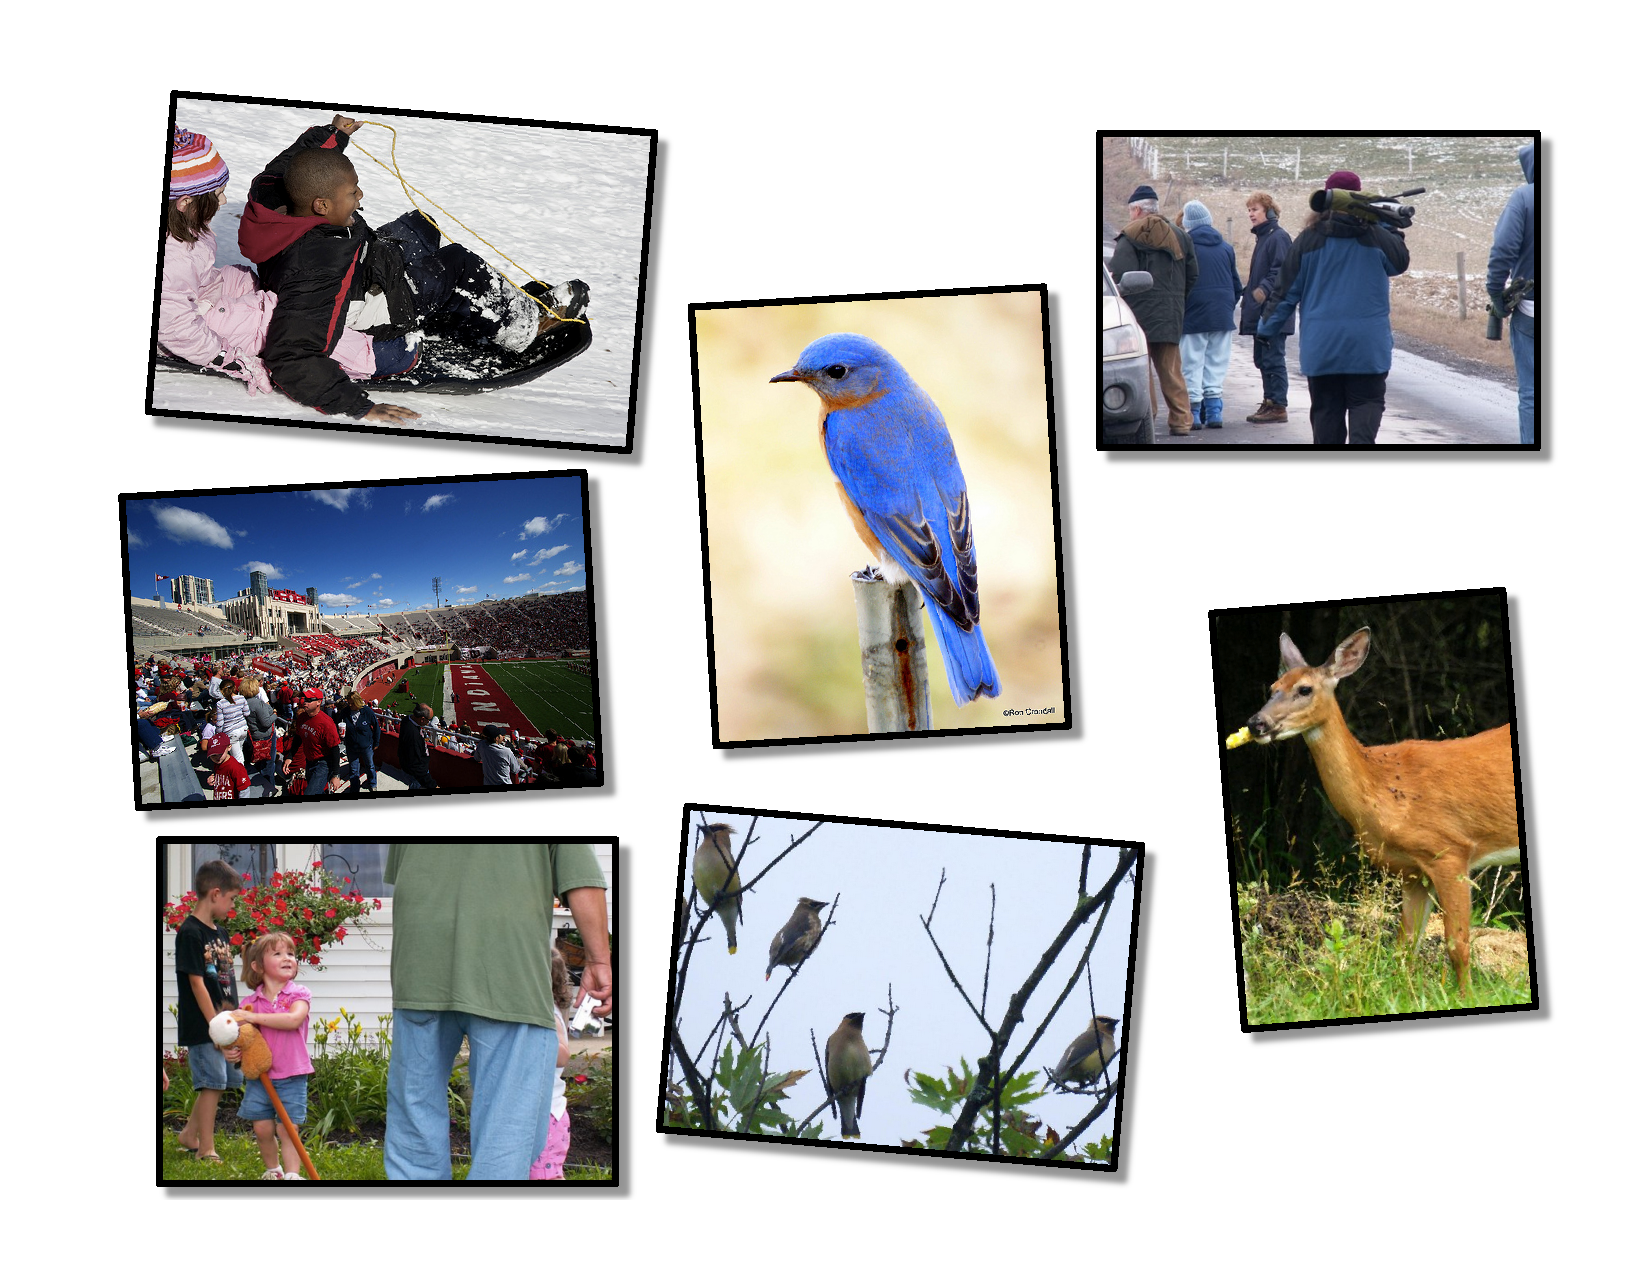
\includegraphics[width=0.42\textwidth,clip,trim=2cm 1cm 1cm 1cm]{figs/natural-images.pdf}
\end{center}
\caption{Many Flickr images contain evidence about the state of the natural world, including
that there is snow on the ground at a particular place and time, that a particular species of bird or animal is present,
and that particular species of plants are flowering.}
\label{fig:nature}
\vspace{-12pt}
\end{figure}

For instance, many (if not most) outdoor images contain some
information about the state of the natural world, such as the weather
conditions and the presence or absence of plants and animals
(Figure~\ref{fig:nature}).  The billions of images on social media
sites could be analyzed to recognize these natural objects and
phenomena, creating a new source of data to biologists and ecologists.
Where are marigolds blooming
today, and how is this geospatial distribution different from a year
ago? Are honeybees less populous this year than last year? Which day
do leaves reach their peak color in each county of the northeastern
U.S.?  These questions can be addressed to some extent by traditional
data collection techniques like satellite instruments, aerial surveys,
or longitudal manual surveys of small patches of land, but none of
these techniques allows scientists to collect fine-grained data at
continental scales: satellites can monitor huge areas of land but cannot 
detect fine-grained features like blooming flowers, while manual surveys
can collect high-quality and fine-grained data only in a small plot of land.
Large-scale analysis of photos on social media
sites could provide an entirely new source of data at a fraction of the cost
of launching a satellite or hiring teams of biologist observers.

The idea of using crowd-sourced data for science and other purposes is
of course not new. Citizen science projects have trained  groups
of volunteers to recognize and report natural phenomena (like bee
counts~\cite{greatsunflower}, bird sightings~\cite{ebirds}, and
snowfall~\cite{king09snowtweets}) near their homes.
Data mining work  has
shown that  social networking sites
like Twitter can 
monitor political opinions~\cite{jin10prediction,digrazia13},
predict financial markets~\cite{bollen11twitter}, track the spread of
disease~\cite{ginsberg09flu}, detect earthquakes~\cite{Sakaki:2010uv}, and monitor weather
conditions~\cite{meteo}. However, the vast majority of this work has
used textual data from micro-blogging sites like Twitter; very few papers have tried to do this with images, despite
the fact that images offer evidence that is richer, less ambiguous,
and much more difficult to fabricate. This is of course because it is
much easier to scan for keywords in Twitter feeds than to
automatically recognize semantic content in huge collections of
images. 
%% In fact, we're aware of only a few papers that have tried to
%% use content analysis of large-scale image collections to observe the
%% physical world. For instance, Leung and Newsam~\cite{Leung:2010wa} used automatic
%% analysis of social image data to infer land use type for a portion of
%% the United Kingdom, while Zhang \textit{et al}~\cite{



In this paper, we test the feasibility of observing the natural world
by recognizing specific types of scenes and objects in large-scale
image collections from social media.  We consider a well-defined but
nevertheless interesting problem: deciding whether there was snow on
the ground at a particular place and on a particular day, given the
set of publicly-available Flickr photos that were geo-tagged and
time-stamped at that place and time. This builds on our early work in
Zhang \textit{et al}~\cite{ecology2012www} which considered a similar
problem, but used only tag information (essentially scanning for
photos that had the tag ``snow'' with some very simple image
processing to remove obvious outliers). Here, we explicitly test
whether large-scale recognition of the image content itself could be
used to do this task.  Of course, snow cover can already be monitored
through satellites and weather stations (although neither of these
data sources is perfect: weather stations are sparse in rural areas
and satellites typically cannot estimate snow cover when it is
cloudy~\cite{modissnow}), so this is not a transformative application
for ecologists in and of itself. Instead, this is an interesting
application for us precisely because fine-grained ground truth is
available, so that we can test the accuracy of crowd-sourced
observations of the natural world, and judge the feasibility of
observing other natural phenomena for which  there are no other possible sources of data.


We initially expected snowy scene recognition to be an easy problem,
in which just looking for large white regions
would work reasonably well.  Surprisingly, amongst the hundreds of
papers on object and scene classification in the literature, we were
surprised to find very few that have explicitly considered detecting
snow. A few papers on scene classification include
snow-related
categories~\cite{XiaoHEOT10,li2007event,li2009totalscene}, while a few
older papers on natural materials
detection~\cite{luo2003spatialcontext,boutell2006semanticfeature}
consider it along with other categories. We test a variety of
recognition techniques on this problem, using a new realistic dataset
of several thousand  images from Flickr with labeled ground
truth.  We find that snow detection in consumer images is 
surprisingly difficult, and we hope this paper and our dataset
will help spark interest in this somewhat overlooked vision problem.
%
We also consider an ecology application where reliable data does not
exist and Flickr image analysis could be potentially quite valuable: estimating the geo-temporal flowering distribution of the
California Poppy.  

%Finally we present some results of applying our
%recognition techniques on geo-tagged and time-stamped images from
%Flickr, in order to estimate the geo-spatial distribution of snow. We
%compare these maps to ground-truth from satellite data.



\hfill \break
\hfill \break
===================================
\hfill \break
\hfill \break
\subsection*{www}


The popularity of social networking websites has grown dramatically
over the last few years, creating enormous collections of
user-generated content online. Photo-sharing sites have become
particularly popular: Flickr and Facebook alone have amassed an
estimated 100 billion images, with over 100 million new images
uploaded every day~\cite{Kremerskothen11}.  People use these
sites to share photos with family and friends, but in the process they
are creating immense public archives of information about the world:
each photo is a record of what the world looked like at a particular
point in time and space.  When combined together, the billions of
photos on these sites combined with metadata including timestamps,
geo-tags, and captions are a rich untapped source of information about
the state of the world and how it is changing over
time.

Recent work has studied how to mine passively-collected data
from social networking and microblogging websites to make estimates
and predictions about world events, including tracking the spread of
disease~\cite{ginsberg09flu}, monitoring for fires and
emergencies~\cite{delongueville09}, predicting product adoption rates
and election outcomes~\cite{jin10prediction}, and estimating aggregate
public mood~\cite{oconnor10mood,bollen11twitter}. In most of these
studies, however, there is either little ground truth available to
judge the quality of the estimates and predictions, or the available
ground truth is an indirect proxy (e.g. since no aggregate public mood
data exists, \cite{oconnor10mood} evaluates against opinion polls,
while~\cite{bollen11twitter} compares to stock market indices).  While
these studies have demonstrated promising results, it is not yet clear
when crowd-sourcing data from social media sites can yield reliable
estimates, or how to deal with the substantial noise and bias in these
datasets. Moreover, these studies have largely focused on textual
content and have not taken advantage of the vast amount of visual
content online.

In this paper, we study the particular problem of estimating
geo-temporal distributions of ecological phenomena using geo-tagged,
time-stamped photos from Flickr.  Our motivations to study this
particular problem are three-fold.  First, biological and ecological
phenomena frequently appear in images, both because photographers take
photos of them purposely (e.g. close-ups of plants and animals) or
incidentally (a bird in the background of a family portrait, or the
snow in the action shot of children sledding).  Second, for the two
phenomena we study here, snowfall and vegetation cover, large-scale
(albeit imperfect) ground truth is available in the form of
observations from satellites and ground-based weather stations.  Thus
we can explicitly evaluate the accuracy of various techniques for
extracting semantic information from large-scale social media
collections.

\begin{figure*}[th]
\begin{center}
\begin{tabular}{ccc}
\textbf{Raw satellite map} & \textbf{Coarsened satellite map} & \textbf{Map estimated by Flickr photo analysis} \\
\fbox{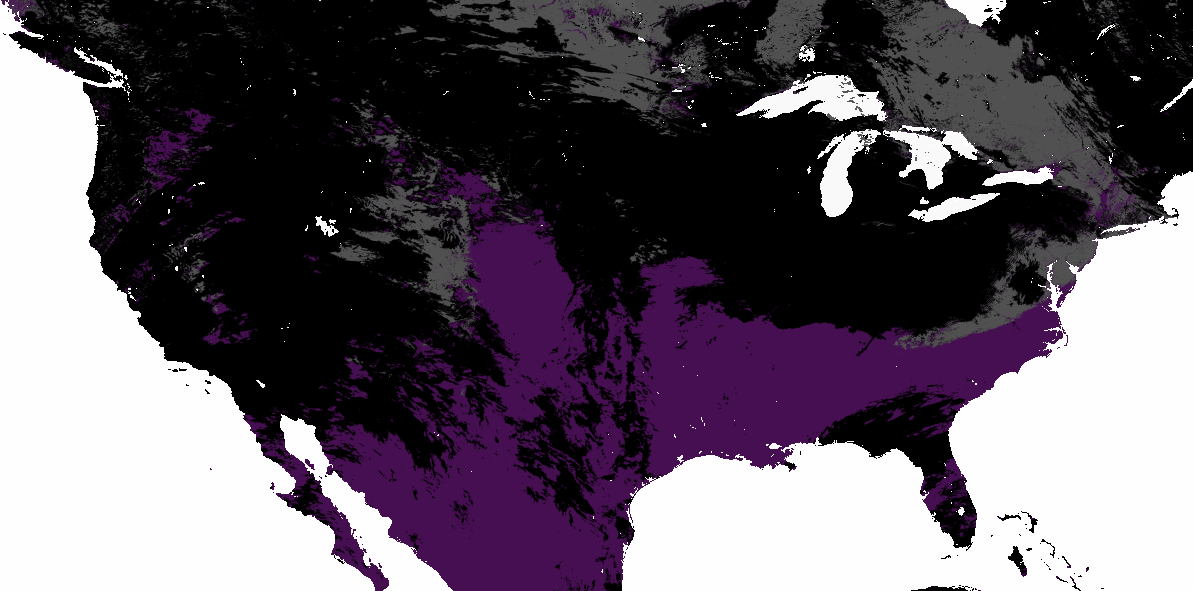
\includegraphics[width=0.23\textheight]{figs/newsat-12212009.png}} &
\fbox{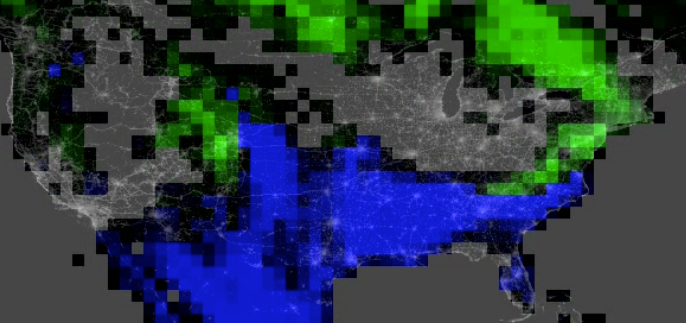
\includegraphics[width=0.23\textheight]{figs/sat-dec212009.png}} &
\fbox{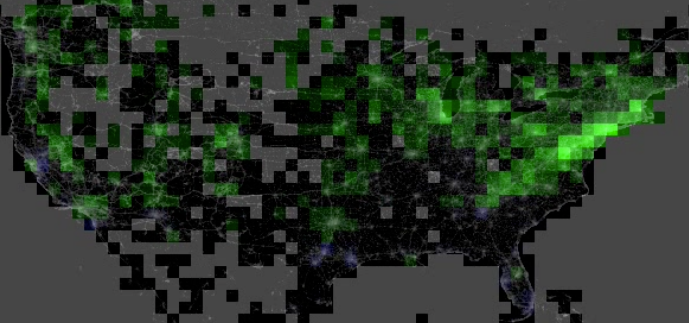
\includegraphics[width=0.23\textheight]{figs/flickr-dec212009.png}} \\
\end{tabular}
\end{center}
\vspace{-6pt}
\caption{Comparing MODIS satellite snow coverage data for North
  America on Dec 21, 2009 with estimates produced by analyzing Flickr
  tags (best viewed on screen in color). \textit{Left:} Original MODIS snow data, where white
  corresponds with water, black is missing data because of cloud
  cover, grey indicates snow cover, and purple indicates no
  significant snow cover.  \textit{Middle:} Satellite data coarsened
  into 1 degree bins, where green indicates snow cover, blue indicates
  no snow, and grey indicates missing data.  \textit{Right:} Estimates
  produced by the Flickr photo analysis proposed in this paper, where
  green indicates high probability of snow cover, and grey and black
  indicate low-confidence areas (with few photos or ambiguous evidence).}
\label{fig:samplemap}
\end{figure*}


Third, while ground truth is available for these particular
phenomena, for other important ecological phenomena (like the geo-temporal distribution of plants and animals) no such data is
available, and social media could help fill this need.
%, and mining data from social media has the potential to fill
%this gap.  
In fact, perhaps no community is in greater need of
real-time, global-scale information on the state of the world than the
scientists who study climate change. Recent work shows that global
climate change is impacting a variety of flora and fauna at local,
regional and continental scales: for example, species of
high-elevation and cold-weather mammals have moved northward, some
species of butterflies have become extinct, waterfowl are losing
coastal wetland habitats as oceans rise, and certain fish populations
are rapidly declining~\cite{ipcc2007climate}. However monitoring these
changes is surprisingly difficult: plot-based studies
involving direct observation of small patches of land yield
high-quality data but are costly and possible only at very small
scales, while aerial surveillance gives data over
large land areas but cloud cover, forests, atmospheric
conditions and mountain shadows can interfere with the observations,
and only certain types of ecological information can be collected from
the air.  To understand how biological phenomena are responding to
both landscape changes and global climate change, ecologists need an
efficient system for ground-based data collection to give detailed
observations across the planet.  A new approach
for creating ground-level, continental-scale datasets is to use
passive data-mining of the huge number of visual observations produced
by millions of users worldwide, in the form of digital images uploaded
to photo-sharing websites.


\xhdr{Challenges.}
There are two key challenges to unlocking the ecological
information latent in these photo datasets. The first is how to recognize 
ecological phenomena appearing in photos and how to map these observations to
specific places and times. Fortunately, modern photo-sharing sites
collect a rich variety of non-visual
information about photos, including metadata recorded by the digital
camera --- exposure settings and timestamps, for example --- as well as
information generated during social sharing  ---
text tags, comments, and ratings, for example. Many sites also
record the
 geographic coordinates of where on Earth a photo was taken, as reported either by a GPS-enabled camera or smartphone, or input manually by the user.
Thus online photos include the ingredients
necessary to produce geo-temporal data about the world,
including information about content (images, tags and comments), and
when (timestamp) and where (geotag) each photo was taken.

The second challenge is how to deal with the biases and noise inherent
in online data. People do not photograph the Earth evenly,
 so there are disproportionate concentrations of
activity near cities and tourist attractions. Photo metadata is often
noisy or inaccurate; for example, users forget to set the clock on
their camera, GPS units fail to find fixes, and users
carelessly tag photos.  Even photos without such errors might be
misleading: the tag ``snow'' on an image might refer to a snow lily or a
snowy owl, while snow appearing in an image might be artificial (as in an indoor zoo exhibit).

\xhdr{This paper.}  In this paper we study how to mine data from
photo-sharing websites to produce crowd-sourced observations of
ecological phenomena.  As a first step towards the longer-term goal of
mining for many types of phenomena, here we study two in particular:
ground snow cover and vegetation cover (``green-up'') data. Both are
critical features for ecologists monitoring the earth's ecosystems.
Importantly for our study, these two phenomena have accurate
fine-grained ground truth available at a continental scale in the form
of observations from aerial instruments like NASA's Terra earth-observing
satellites~\cite{modisveg,modissnow} or networks of ground-based
observing stations run by the U.S. National Weather Service. This
data allows us to evaluate the performance of our crowd-sourced data mining
techniques at a very large scale, including thousands of days of data
across an entire continent.
%This evaluation gives insight into how accurate crowd-sourced 
%observations could be for tracking ecological phenomena for which
%no ground truth exists.
 Using a dataset of nearly 150 million geo-tagged Flickr photos, we
 study whether this data can potentially be a
 reliable resource for scientific research.  An example comparing
 ground truth snow cover data with the estimates produced by our
 Flickr analysis on one particular day (December 21, 2009) is shown in
 Figure~\ref{fig:samplemap}. Note that the Flickr analysis is sparse
 in places with few photographs, while the satellite data is missing
 in areas with cloud cover, but they agree well in areas where both
 observations are present. This (and the much more extensive experimental results presented later in the paper) suggests that Flickr analysis may produce
 useful observations either on its own or as a complement other
 observational sources.


%% More generally, this paper is a step towards answering a more basic
%% question: How reliable could passive mining of social sharing sites be
%% in producing observations of the world?  Analyzing data from social
%% networking and microblogging websites to make estimations and
%% predictions about world events has become a popular research
%% direction, including for example tracking the spread of
%% disease~\cite{ginsberg09flu}, monitoring for fires and other
%% emergencies~\cite{delongueville09}, predicting product adoption and
%% election outcomes~\cite{jin10prediction}, and inferring aggregate
%% public mood~\cite{oconnor10mood,bollen11twitter}. In most of these
%% studies, however, there is either no ground truth to judge the quality
%% of the estimates, or the ground truth that is used is an indirect
%% proxy (e.g. since no aggregate public mood data exists,
%% \cite{oconnor10mood} evaluates against opinion polls,
%% while~\cite{bollen11twitter} compares to stock market indices). In
%% contrast, for predicting some ecological phenomena like vegetation and
%% snow cover, we have daily, dense ground-truth data for the entire
%% globe in the form of satellite observations.

To summarize, the main contributions of this paper include: 

\begin{packed_itemize}
\item[---] introducing the novel idea of mining photo-sharing sites for
  geo-temporal information about ecological phenomena, 
\item[---] introducing several techniques for deriving crowd-sourced
  observations from noisy, biased data using both visual and textual tag analysis, and
\item[---] evaluating the ability of these techniques to accurately measure
  these phenomena, using dense large-scale ground truth.
\end{packed_itemize}





